\chapter{脉搏波时域描述特征集的构建及分析处理}
\section{引言}
第三章已经对脉搏波的描述特征参数进行了介绍,本章选取了其中的部分参数构成了基本机器学习的输入数据集。
本章对这部分特征数据按机器学习的一般要求进行了相关处理及准备工作。

\section{脉搏波时域描述特征集的构建}
在第三章基于波形的新型时域特征参数的基础上,本研究选取了其中的部分参数作为后续建立子痫前期识别模型的输入特征集合。出于不同的设计考量,本研究共构建了三个相互独立的脉搏波描述特征集作为
特定模型的训练输入数据。本文的后续分析工作暂未对这三个脉搏波描述特征集进行交叉合并处理。

\subsection{新型时域波形描述特征集合}

如\autoref{fig:road}及\autoref{fig:point}所示,在对脉搏波进行抽象之后,对脉搏波的描述通过选取一系列特殊的基本点$Q$,再借助基于这些选中的基本点的描述指标完成对脉搏波的描述。在使用这种方法对脉搏波进行描述时,
往往需要选取设置多个这样的点,因此,最后的描述结果通常是以向量的形式存在的,即脉搏波波形特征描述向量。换言之,只要确定了选取基本描述点的原则,就可以得到一系列的基于线段、曲线长度、斜率、弧度及面积等指标的
脉搏波波形特征描述向量。本研究使用了三类基本描述点的相关指标。

一、左视类指标

左视类指标(Left View Index)是以脉搏波上升支起点为中心,将上升支起点与脉搏波峰值点与水平线的夹角等分成10份。这些等分线与脉搏波的交点即为基本描述点,如\autoref{fig:lv}所示。
\begin{figure}[htbp]
  \centering
  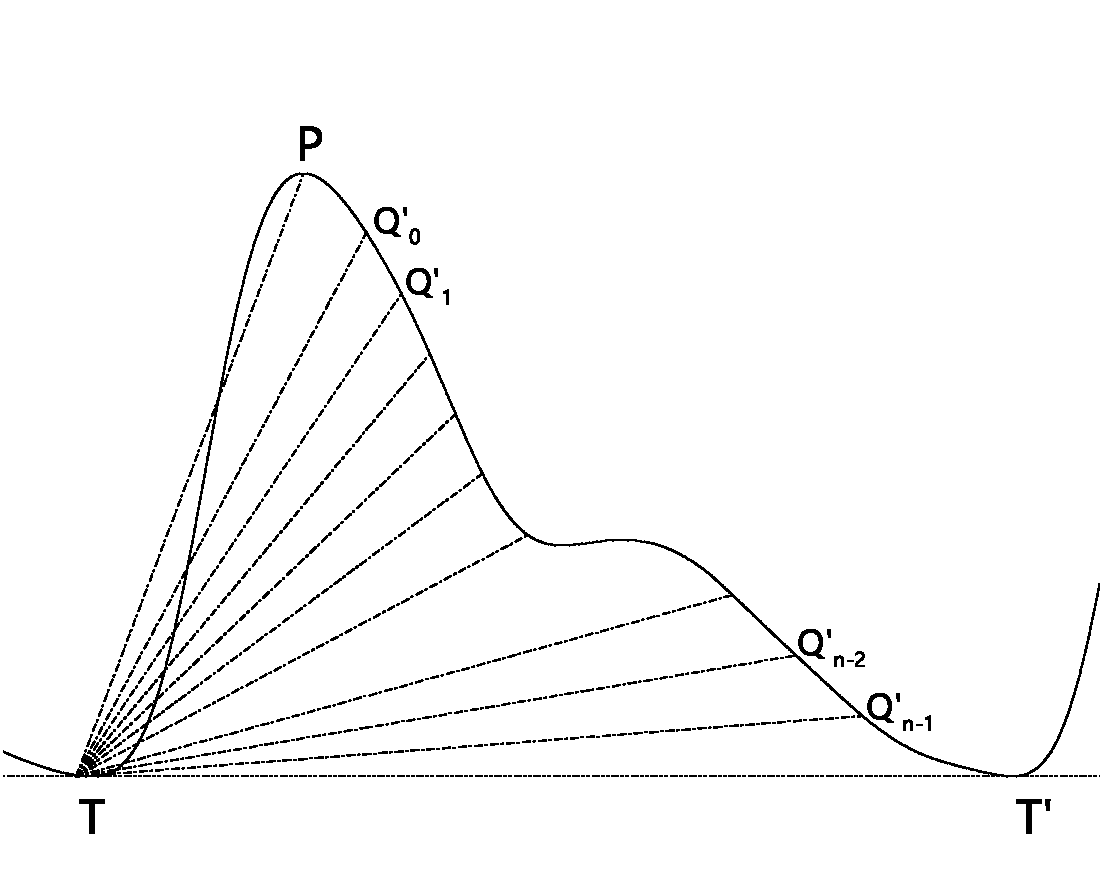
\includegraphics[width=.6\linewidth]{features/lv}
  \caption{\label{fig:lv}左视类指标示意}
\end{figure}

二、中视类指标

中视类指标(Center View Index)是以脉搏波波峰在水平线上的映射点为中心,将上升支与下降支分别等分成10份。这些等分线与脉搏波的交点即为基本描述点,如\autoref{fig:cv}所示。
\begin{figure}[htbp]
  \centering
  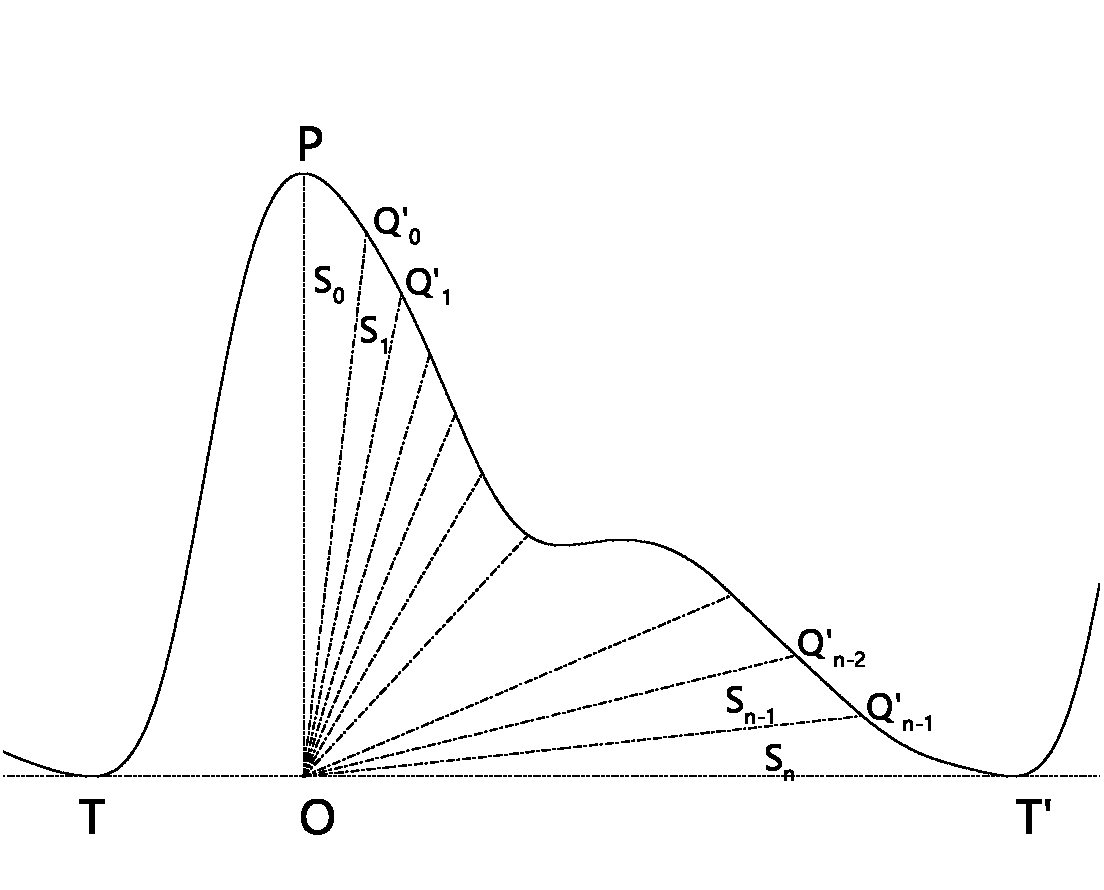
\includegraphics[width=.6\linewidth]{features/cv}
  \caption{\label{fig:cv}中视类指标示意}
\end{figure}

三、分层类指标

分层类指标(Scaled View Index)是将脉搏波峰值等分为10份后,过各等分点作水平线,取各水平线与上升支与及下降支的交点即为基本描述点,如\autoref{fig:sv}所示。
\begin{figure}[htbp]
  \centering
  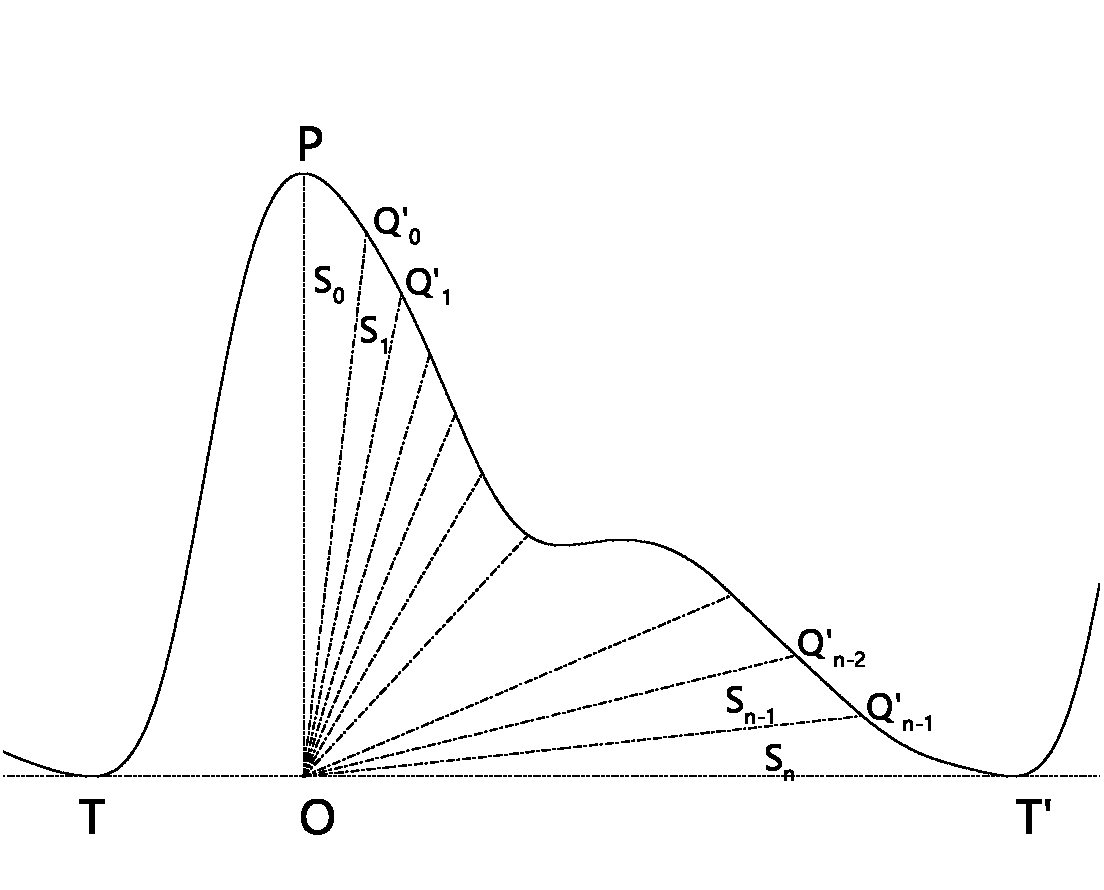
\includegraphics[width=.6\linewidth]{features/cv}
  \caption{\label{fig:sv}分层类指标示意}
\end{figure}

基于以上基本点得到,可以分别得到基于线段、曲线长度、斜率、弧度及面积等指标的脉搏波波形特征描述向量,这些指标如表\autoref{tab:allfeatures}所示。最后需要指出的是,以上特征参数的计算都是在脉搏波波形标准化之后进行的。
出于方便计算的考虑,所有的脉搏波波形幅值被调整缩放至[0,1000]区间内,其中脉搏波波形上升支与下降支分别进行了线性变换处理。\autoref{tab:allfeatures}所示的这些时域特征被统一称为\textbf{脉搏波时域特征集\Rnum{1}}。
\begin{center}
  \zihao{5}
  \begin{longtable}{m{4cm}<{\centering}m{2cm}<{\centering}m{8.5cm}<{\centering}}
    \caption{本研究使用的所有PPG时域指标一览}\\
    \label{tab:allfeatures}\\
        \toprule
        \textbf{名称}&\textbf{缩写}&\textbf{意义}\\
        \midrule
        \endfirsthead
        \caption[]{(续)}\\
        \midrule
        \textbf{名称}&\textbf{缩写}&\textbf{意义}\\
        \midrule
        \endhead 
        \midrule
        \endfoot
        \bottomrule
        \endlastfoot
        左视斜率    &   LVS    &   各等分线所对应的直线斜率   \\
        左视上升支交点坐标 & LVLR & 等分线与脉搏波波形上升支交点横坐标 \\
        左视下降支交点坐标 & LVLF & 等分线与脉搏波波形下降支交点横坐标 \\
        左视上升支交点距离 & LVRR & 等分线与脉搏波波形上升支交点与波形起点距离 \\
        左视下降支交点距离 & LVRF & 等分线与脉搏波波形下降支交点与波形起点距离 \\
        左视交点坐标差 & LVD & 左视上升支交点坐标与左视下降支交点坐标之差 \\
        左视上升支弧长 & LVALR & 脉搏波波形上升支被等分线分割的各区间弧长 \\
        左视下降支弧长 & LVALF & 脉搏波波形下降支被等分线分割的各区间弧长 \\
        中视上升支交点坐标 & CVLR & 等分线与脉搏波波形上升支交点横坐标 \\
        中视下降支交点坐标 & CVLF & 等分线与脉搏波波形下降支交点横坐标 \\
        中视上升支交点距离 & CVRR & 等分线与脉搏波波形上升支交点与峰值水平映射点距离 \\
        中视下降支交点距离 & CVRF & 等分线与脉搏波波形下降支交点与峰值水平映射点距离 \\
        中视交点坐标差 & CVD & 中视上升支交点坐标与中视下降支交点坐标之差 \\
        中视上升支弧长 & CVALR & 脉搏波波形上升支被等分线分割的各区间弧长 \\
        中视下降支弧长 & CVALF & 脉搏波波形下降支被等分线分割的各区间弧长 \\
        中视上升支面积 & CVAR & 脉搏波波形上升支被等分线分割的各区域面积 \\
        中视下降支面积 & CVAF & 脉搏波波形下降支被等分线分割的各区域面积 \\
        分层上升支交点坐标 & SVLR & 等分线与脉搏波波形上升支交点横坐标 \\
        分层下降支交点坐标 & SVLF & 等分线与脉搏波波形下降支交点横坐标 \\
        分层上升支面积 & SVAR & 脉搏波波形上升支被等分线分割的各区域面积 \\
        分层下降支面积 & SVAF & 脉搏波波形下降支被等分线分割的各区域面积 \\
        分层面积 & SVAT & 脉搏波波形整体被等分线分割的各区域面积 \\
        分层上升支交点距离 & SVRR & 等分线与脉搏波波形上升支交点与峰值水平映射点距离 \\
        分层下降支交点距离 & SVRF & 等分线与脉搏波波形下降支交点与峰值水平映射点距离 \\
        分层交点坐标差 & SVD &  分层上升支交点坐标与分层下降支交点坐标之差\\
        分层上升支弧长 & SVALR & 脉搏波波形上升支被等分线分割的各区间弧长 \\
        分层下降支弧长 & SVALF & 脉搏波波形下降支被等分线分割的各区间弧长 \\
        分层上升支斜率 & SVSR & 等分线与脉搏波波形上升支交点与脉搏波峰值水平映射点所形成直线的斜率\\
        分层下降支斜率 & SVSF & 等分线与脉搏波波形下降支交点与脉搏波峰值水平映射点所形成直线的斜率 \\
        上升支标准化斜率 & STDKR & 标准化脉搏波上升支波形至[0-1000]时使用的斜率 \\
        上升支标准化截距 & STDBR & 标准化脉搏波上升支波形至[0-1000]时使用的截距 \\
        下降支标准化斜率& STDKF & 标准化脉搏波下降支波形至[0-1000]时使用的斜率 \\
        下降支支标准化截距 & STDBF & 标准化脉搏波上升支波形至[0-1000]时使用的截距 \\
  \end{longtable}
\end{center}

\subsection{原始波形采样值}

第三章已经阐述过,脉搏波信号的原始采样值可以看成向量维数与采样点数相同的特殊脉搏波波形特征描述向量。从这个角度而言,原始采样值可以直接用作描述波形的时域特征。
其中,原始采样值已经按照上小节方法被标准化至[0-1000]区间内。考虑到不同波形的时长有差异,即波形的采样点数可能不同,原始波形的采样点数被重采样调制至100。
这种基于原始波形采样值的脉搏波时域特征被称为\textbf{脉搏波时域特征集\Rnum{2}}。

\subsection{波形间差异描述特征集合}
波形间差异描述特征集合目前特征参数较少,仅包括第三章中介绍的相关系数、弗朗明歇距离及包络面积差三种。这三种特征在使用时分别按照只计算相邻两个波形差异及以前10个波形为模板得到标准波形后,后续所有波形与标准波形差异性的比较。
这些基于脉搏波波形间差异的时域特征参数被称为\textbf{脉搏波时域特征集\Rnum{3}}。

\section{脉搏波时域描述特征集的分析处理}
在应用上述脉搏波时域特征集构建机器学习进行分析工作之前,还需按照机器学习的通用方法进行一定的处理。这部分的工作包括数据集划分、特征缩放、特征降维等。
\subsection{数据集的划分}
在大多数机器学习的案例里,在开始模型训练之前将原始数据集划分为训练集与测试集是必不可少的一个步骤。其中,训练集用来生成特定的机器学习模型,而测试集则用来评估该模型的泛化能力。
本研究后续内容涉及到多种机器学习模型的训练,为科光进行各模型性能评估,需要保持训练集与测试集的一致性。因此,本研究采取了如下策略:

一、分层抽样

由于本研究的特征数据样本数据规模较小(被试人员79名,整理得到有效波形7900多个),直接使用纯随机抽样有可能导致抽样偏差,影响最终模型的准确性\cite{Aurélien2018}。
因此,在划分测试集时,针对数据样本按其对应的被试孕妇是否患有子痫,分别按照训练集与测试集4:1的比例分别进行抽样,两次抽样结果合并后才形成
最终的训练集与测试集。

二、固化抽样结果

上述分层抽样仅运行一次,其划分结果被保存,后续所有模型的训练均使用这次抽样结果,不再调整。

另一方面,由于本研究的研究目标是探寻脉搏波与子痫前期之间的关系,但前面所准备的特征数据是基于单个脉搏波波形的,而一条脉搏波数据对应着多个脉搏波波形数据。
因此,本研究采用了以下两种划分数据的方式:

一、按照全部波形数据分层抽样

这种抽样方式将单个脉搏波波形作为最小划分单位,这也意味着同一个被试孕妇的实验数据可对应多个“数据样本”。同一被试的不同脉搏波波形可能会被分别划分进训练集与测试集之中。

二、按被试人员分层抽样

这种抽样方式仅以被试是否患有子痫前期为标准进行分层抽样。同一被试的脉搏波波形只会出现在训练集或测试集之中。这也意味着测试集中的数据样本将会是模型训练阶段完全未见的。

\subsection{特征缩放}
  在大多数情况下,原始数据的特征在数值属性出现较大的比例差异会导致机器学习模型的性能下降、表现欠佳\cite{Aurélien2018}。因此,需要对特征数值的分布进行一定的调整使其能够满足具体模型算法的输入要求。
  一般的处理原则是同比例缩放所有属性,常见的方法有归一化与标准化两类。归一化亦称为最小-最大缩放,可将所有数据属性值同比例映射至[0,1]区间内。
  而标准化的过程则是所有数据的属性值先减去平均值后,再除以样本方差,标准化处理之后得到的数据属性符合正态分布。

\subsection{特征降维}
事实证明,机器学习模型的训练速度随着训练数据的特征数量增加而降低,这也就是通常而言的维数诅咒或维数灾难。因此,一种可行的策略在构建模型时尽可能只使用“与预期结果最相关的”、“最重要的”特征,即按照特征的贡献度对
原始数据集进行降维处理。但需要注意的是,数据降维在加速训练的同时,通常也会导致系统性能的下降。从这个角度说,特征降维是机器学习过程中的一个可选项而非必选项。特征降维在训练模型前后均可进行。在相关模型生成前的特征降维
主要依赖于特征数据属性值的分布特性进行取舍;在模型生成后的特征降维主要依赖于特征属性对模型的贡献程度进行取舍。

本小节使用了U检验对脉搏波时域特征集\Rnum{1}上的各特征属性在数据标签(是否患有子痫)进行了检验,其中p值$\> 10^{-4}$的特征属性如\autoref{tab:utest}所示,p值$> 0.05$的特征未参与后续模型的训练过程。

\begin{center}
  \zihao{5}
  \begin{longtable}{m{2.5cm}<{\centering}m{2cm}<{\centering}m{2.5cm}<{\centering}m{2cm}<{\centering}m{2.5cm}<{\centering}m{2cm}<{\centering}}
    \caption[脉搏波时域特征集\Rnum{1}数据特征的U检验结果]{脉搏波时域特征集\Rnum{1}数据特征的U检验结果。p值> 0.05的结果被加粗显示。}\\
    \label{tab:utest}\\
        \toprule
        \textbf{特征}&\textbf{p值}&\textbf{特征}&\textbf{p值}&\textbf{特征}&\textbf{p值}\\
        \midrule
        \endfirsthead
        \caption[]{(续)}\\
        \midrule
        \textbf{特征}&\textbf{p值}&\textbf{特征}&\textbf{p值}&\textbf{特征}&\textbf{p值}\\
        \midrule
        \endhead 
        \midrule
        \endfoot
        \bottomrule
        \endlastfoot
          LVLR\_9  &  0.004 &  CVLF\_1  &  \textbf{0.068} &  SVRR\_2  &  0.027 \\
          LVLF\_1  &  \textbf{0.27}  &  CVLF\_2  &  0.038 &  SVRR\_3  &  0.001 \\
          LVRR\_6  &  0.002 &  CVRF\_4  &  \textbf{0.44}  &  SVRR\_4  &  0.001 \\
          LVRR\_7  &  \textbf{0.387} &  CVD\_1   &  \textbf{0.159} &  SVD\_2   &  0.009 \\
          LVD\_1   &  0.022 &  CVD\_2   &  0.024 &  SVD\_3   &  \textbf{0.65}  \\
          LVD\_2   &  0.006 &  CVALF\_6 &  0.02  &  SVALR\_2 &  \textbf{0.078} \\
          LVALR\_4 &  0.013 &           &        &  SVALR\_3 &  0.001 \\
          LVALR\_5 &  \textbf{0.063} &           &        &           &               
  \end{longtable}
\end{center}

\section{小结}
本小节在已经脉搏波预处理过程的基础上完成了脉搏波时域特征集合的构建,包括基于脉搏波波形特征描述向量、原始采样值及脉搏波波形差异值等三大类。
此外,本小节也完成了机器学习的数据集划分、特征缩放及特征降维等部分的工作。